\documentclass{article}
\author{
    Epidemiological Modelling Unit,
    \\ School of Public Health and Preventive Medicine,
    \\ Monash University
}
\usepackage{graphicx}
\usepackage{biblatex}
\usepackage{threeparttable}
\usepackage{tabularx}
\usepackage{alphabeta}
\usepackage{amsmath}
\usepackage{caption} \captionsetup[table]{singlelinecheck=false}
\usepackage[labelfont=bf]{caption}
\usepackage[left=2.5cm,right=2.5cm]{geometry}
\bibliography{../../references/emu_library}

\title{Modelling methods, Kiribati application}

\begin{document}

\maketitle

% This file describes the general structure of some of our tb_dynamics models.

\section{Model Structure}

\subsection{General features}

We use a deterministic compartmental model including six types of compartments that represent 
different states of infection and disease. The model uses the same conceptual approach and similar 
assumptions to previously published models \cite{trauer-2017, ragonnet-2019, ragonnet-2021, ragonnet-2022}. 
Here we describe the model structure without treatment compartment and related factors. 
\newline
A susceptible compartment (S) is used to represent individuals who have 
never been infected with \emph{Mycobacterium tuberculosis (M.tb)}. Latent TB infection (LTBI) is modelled 
using two successive compartments: early latent (E) and late latent (L) to capture the declining risk of 
disease progression over time from infection \cite{ragonnet-2017}. The active disease compartment (I) represents 
individuals who have progressed to the active stage of TB disease. Diseased individuals who recover 
through self-cure progress directly to the recovered compartment (R).
\newline
Non-TB-related mortality is modelled by applying death rates to all model compartments. In addition, 
disease-specific mortality is implemented by applying increased mortality rates to the active disease 
compartments (I).
\newline
Reinfection occurs in the model in two different ways. First, latently infected individuals may be 
reinfected, with this process modelled using a flow from the late latent (L) to the early latent 
compartment (E). Second, individuals who have recovered from TB disease may be reinfected and 
return to the early latent compartment. The structure of our model allows for differential risk of 
infection for the currently and previously infected individuals, compared to the infection-naive 
individuals.
\begin{figure}[!htp]
    \vspace*{-1cm}
    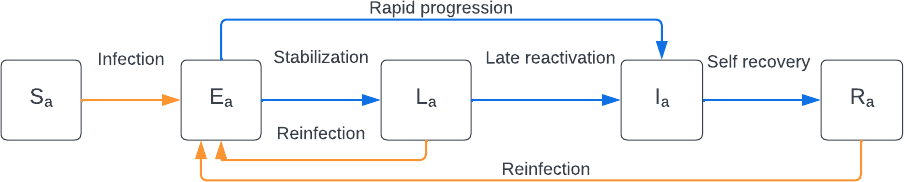
\includegraphics[width=\textwidth,height=\textheight,keepaspectratio]{images/model.png}
    \caption{Illustration of the model structure. 
    Boxes represent the different compartments types: susceptible (S), early latent (E), late latent (L), infectious (I), and recovered (R).
    The subscript indicates that compartments are stratified by age (a).}
    \label{fig:model}
\end{figure}

\subsection{Stratification by age}
The model is stratified using five categories: 0-4, 5-14, 15-34, 35-49 and 50+ years old. We assume 
heterogeneous mixing by age using an age-specific contact rate matrix. Since no local estimates of 
contact patterns by age were available for the Marshall Islands, we used a contact survey conducted in 
the Fijian population and adjusted the estimates to account for age distribution differences between
the two countries.



\begin{figure}[ht]
    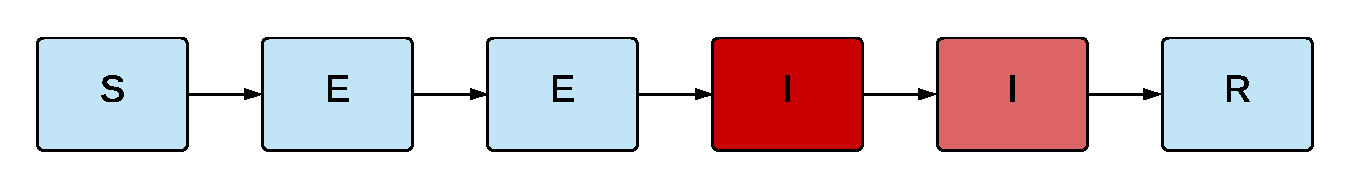
\includegraphics[width=\textwidth]{../../tex_descriptions/models/sm_sir/sm_sir_seir.pdf}
    \caption{Unstratified compartmental model structure. S = susceptible, E = exposed, I = active, R = recovered/removed. Depth of pink/red shading indicates the infectiousness of the compartment.}
    \label{fig:seeiir}
\end{figure}

\section{Model stratification}
\subsection{Model stratification}
% Note that this will vary for every application, so will need to be edited - not sure of how best to manage this:
All compartments of the base compartmental structure were stratified by age, location and organ status:\linebreak
Age
\begin{itemize}
    \item Zero to 14 years
    \item 15 to 24 years
    \item 25 to 49 years
    \item 50 to 69 years
    \item 70 years and above
\end{itemize}
Location
\begin{itemize}
    \item South Tarawa
    \item Other location
\end{itemize}
Organ status
\begin{itemize}
    \item Pulmonary smear-posivtive
    \item Pulmonary smear-negative
    \item Extrapulmonary
\end{itemize}

\subsection{Births and deaths}
Births are modelled using time-variant crude birth rates that are multiplied by the modelled population 
size to determine the number of newborn individuals entering the model at each time. A time-variant 
and age-specific rate or non-TB-related mortality applies to all model compartments to simulate 
deaths from other causes than TB. We use estimates from the UN population division to inform the 
birth and mortality rates.
We also apply additional death rates to the compartments I and T to reflect mortality induced by TB 
disease.
\subsection{M.tb Tranmission}
We use different levels of susceptibility to infection for individuals who are currently latently infected 
with M.tb or have recovered from active TB, as compared to infection-naive individuals. The effect of 
BCG vaccination is captured by reducing the susceptibility to infection of individuals under the age of 
30 years old. We assume a 70\% reduction in the susceptibility of BCG-vaccinated children under the 
age of 15 years old. A linear function is used to reflect the progressive loss of BCG immunity 
between the age of 15 and 30 years old. 
\section{Infectious seed}
The infectious seed value is assigned to the early infectious compartment.
This value is subtracted from the total modelled population and assigned to the susceptible compartment, while all other compartments are assigned a starting value of zero.
This process is undertaken before age stratification is applied,
with the stratification process then splitting these values proportionately according to the starting age distribution of the population.

\section{Progression Parameters}
\subsection{Progression from latent to active TB}
We use the estimates reported in Ragonnet et al. to inform the modelled dynamics of activation from 
latent to active TB. These parameters vary by age, and a multiplier is used to 
incorporate uncertainty around the progression rates
\subsection{Effect of diabetes}
The model is not stratified by diabetes status. Instead, we model the effect of diabetes type 2 by 
increasing the rates of progression from latent to active TB using age-specific multipliers. For each 
age group, the value of the diabetes-effect multiplier depends on the age-specific proportion of 
diabetic individuals and the relative rate of TB reactivation for diabetic individuals compared to non-diabetic individuals.
\subsection{Natural history flows}
We use the estimates reported in Ragonnet et al. to model the rate of TB mortality in the absence of 
treatment and the rate of self-recovery. We use different rates of untreated TB mortality and self-recovery for smear-positive TB compared to smear-negative TB. The TB mortality and self-recovery 
rates associated with extrapulmonary TB are assumed to be the same as those of smear-negative TB.
\subsection{Passive case detection of active TB}
The detection rate is defined as the rate of progression from the active disease to the treatment 
compartment, as all detected individuals are assumed to be started on treatment at diagnosis in our 
model. This rate is calculated by multiplying the screening rate with the diagnostic test sensitivity. 
The screening rate can be interpreted as the reciprocal of the average time that diseased individuals 
take to seek care. The diagnostic sensitivity varies according to the organ status to reflect the relative 
differences in the difficulty to diagnose smear-negative TB and extrapulmonary TB, as compared to 
smear-positive TB.
We use a time-variant function to model the screening rate in order to capture detection improvements 
over time.
\subsection{Treatment outcomes}
Treated individuals can experience three different treatment outcomes: treatment success, relapse or 
death. The rate of treatment-induced recovery \phi{} is set to the reciprocal of the duration of a 
completed treatment course. We then use the observed treatment success proportion (often referred to 
as “treatment success rate”) as model input. In our model, it is calculated from \(TSR = \frac{\phi}{\phi + \rho + \mu_{\tau} + \mu^{'}}\){}, 
where \rho{} is the relapse rate, \({\mu_{\tau}{}}\) is the excess mortality rate of individuals on TB treatment, and \mu is the 
non-TB-related mortality rate. Finally, we calculate the respective values of {\rho}{} and \({\mu_{\tau}{}}\) using the 
observed proportion of deaths among all negative treatment outcomes, denoted \pi{}. We have \({\pi = \frac{\mu_{\tau} +\mu}{\rho + \mu_{\tau} + \mu}}\){} that we inject into the \({TSR}\) equation.


\section{Modelled Intervention}
\subsection{Population-based screening and treatment of LTBI}
Mass LTBI screening and treatment is implemented as part of the intervention conducted in South Tarawa in 
2022. This is modelled by making latently infected individuals (from E and L) transition to the 
recovered compartment (R). The rate associated with these flows is obtained by multiplying the LTBI 
screening rate with the sensitivity of the LTBI test employed and the individual-level efficacy of 
preventive treatment. The LTBI screening rate is implemented as a time-variant parameter that is 
stratified by location
\subsection{Active case finding}
Active case finding (ACF) is implemented to simulate the interventions linked to the detection of 
individuals with active TB implemented in South Tarawa. This is modelled by 
implementing an additional transition flow from compartment I to compartment T. The rate associated 
with this flow is obtained by multiplying the location-specific ACF screening rate with the sensitivity 
of the detection algorithm used for the ACF intervention. The ACF screening rate is implemented as a 
time-variant parameter.
\subsection{Calculation of the screening rates}
To simulate the interventions, we apply a positive rate of ACF and/or LTBI screening over the 
intervention periods. The screening rates are determined such that the modelled total proportion of the 
population screened corresponds to the true population proportion screened. The screening rate is set 
equal to \(-log(1 - coverage)\) for the year during which the intervention is implemented, where 
\(coverage\) is the total proportion of the population screened by the intervention. 
\section{Parameters}
\section{Parameters}
\subsection{Non-age-stratified parameters}

\begin{longtable}[ht]{| >{\raggedright}p{4cm} | >{\raggedright}p{3cm} | p{6.8cm} |}
    \hline
    Parameter & Value & Rationale \\
    \endfirsthead
	\multicolumn{3}{c}{continuation of parameters table}\\
    \endhead
    \hline Incubation period & Calibration parameter, truncated normal distribution, mean 6.1 days, standard deviation 0.8 days & Prior distribution taken from marginal posterior distribution from 2020 analysis \\
    \hline
    Proportion of incubation period infectious & 50\% & Infectiousness is considered to be present throughout a considerable proportion of the incubation period, based on analyses of confirmed source-secondary pairs \cite{RN23} and early findings that the incubation period was similar to the serial interval \cite{RN7}. The study of source-secondary pairs was also the primary reference cited by a review of the infectious period that identified studies that quantified the pre-symptomatic period, which concluded that the median pre-symptomatic period could range from less than one to four days \cite{RN14}. \\
    \hline
    Active period (regardless of detection/isolation, for clinical strata 1 to 3) &
    Calibration parameter, truncated normal distribution, mean 6.4 days, standard deviation 0.7 days &
    Prior distribution taken from marginal posterior distribution from 2020 analysis \\
    \hline
    Proportion of infectious period before isolation or hospitalisation can occur & 
    0.333 &
    Assumed \\
    \hline
    Disease duration prior to admission for hospitalised patients not critically unwell (i.e. early active sojourn time, stratum 4) &
    7.7 days &
    Mean value from ISARIC cohort, as reported on 4\textsuperscript{th} October 2020 in Table 6 \cite{RN22}, and similar to the expected mean from earlier reports from ISARIC \cite{RN16}. This cohort represents high-income countries better than low and middle-income countries, with the United Kingdom contributing data on the greatest number of patients, followed by France. Earlier estimates of this quantity from China included 4.4 days \cite{RN7}. \\
    \hline
    Duration of hospitalisation if not critically unwell (late active sojourn time, stratum 4) &
    7.8 days &
    FluCAN monthly Covid Epi Report to CDNA, 30\textsuperscript{th} August 2020 \\
    \hline
    ICU duration (late active sojourn time, stratum 5) & 5.9 days &
    SPRINT-SARI Australia Project \\
    \hline
    Duration of time prior to ICU for patients admitted to ICU & 
    10.5 days & 
    Calculated as the sum of the time from symptom onset to hospital admission (7.7 days above) plus the duration from hospital admission to ICU admission reported by October ISARIC report (2.8 days) \cite{RN22}. \\
    \hline
    Relative infectiousness of persons admitted to hospital or ICU & 0.2 & Assumed \\
    \hline
    Relative infectiousness of identified persons in isolation & 0.2 & Assumed \\
    \hline
    Clinical effectiveness of one vaccine dose & 0.49 & Mean of one dose effectiveness for BNT162b2 and ChAdOx1 reported in www.medrxiv.org/content/ 10.1101/2021.08.18.21262237v1 \\
    \hline
    Clinical effectiveness of full course of vaccination & 0.775 & Mean of full course effectiveness for BNT162b2 and ChAdOx1 reported in www.medrxiv.org/ content/10.1101/2021.08.18.21262237v1 \\
    \hline
    Proportion of effect of vaccination mediated through prevention of infection & 0.95 & Similar estimates for clinical effectiveness and effectiveness in preventing transmission \\
    \hline
    Reduction in infectiousness of one vaccine dose & 0.56 & Mean of one dose effectiveness for BNT162b2 and ChAdOx1 reported in www.medrxiv.org/content/ 10.1101/2021.08.18.21262237v1 \\
    \hline
    Reduction in infectiousness of full course of vaccination & 0.77 & Mean of full course effectiveness for BNT162b2 and ChAdOx1 reported in www.medrxiv.org/content/ 10.1101/2021.08.18.21262237v1 \\
    \hline    
	\caption{\textbf{Universal (non-age-stratified) model parameters.} Point estimates are used as model parameters except where ranges are indicated in calibration parameter table below in calibration table. Note that all vaccination-related parameters pertain specifically to Delta.}
	\title{Universal model parameters.}
	\label{tab:params}
\end{longtable}

\newpage
\printbibliography

\end{document}
